% The Critical Line Algorithm as implemented in cvxcla
%
% This paper documents the algorithm implemented in src/cvxcla/cla.py
% (with supporting modules first.py, operators.py and types.py).
%
% Build with:  pdflatex cla.tex   (no bibliography tool required)

\documentclass[11pt]{article}

\usepackage[utf8]{inputenc}
\usepackage[T1]{fontenc}
\usepackage{amsmath, amssymb}
\usepackage{bm}
\usepackage{geometry}
\usepackage{graphicx}
\usepackage{hyperref}
\usepackage{booktabs}
\usepackage{xcolor}
\usepackage[round,authoryear]{natbib}

% The algorithm listing below is typeset with only base LaTeX (a boxed minipage
% plus nested enumerate), so the paper builds without the algorithm/algorithmicx
% packages (algorithm.sty / algpseudocode.sty), which are not present in every
% TeX distribution.

\geometry{margin=1in}
\hypersetup{colorlinks=true, linkcolor=blue!50!black, urlcolor=blue!50!black,
  citecolor=blue!50!black}

% --- notation shortcuts -------------------------------------------------
\newcommand{\R}{\mathbb{R}}
\newcommand{\Sig}{\Sigma}
\newcommand{\F}{\mathcal{F}}        % free set
\newcommand{\B}{\mathcal{B}}        % blocked set
\newcommand{\Sset}{\mathcal{S}}     % active inequality-row set
\newcommand{\lb}{\ell}              % lower bound
\newcommand{\ub}{u}                 % upper bound
\newcommand{\trans}{^{\mathsf{T}}}
\newcommand{\inv}{^{-1}}
\DeclareMathOperator*{\argmax}{arg\,max}
\DeclareMathOperator*{\argmin}{arg\,min}

% --- repository links ---------------------------------------------------
% \srcfile{url-path}{display}: a clickable link to a file in the repository.
% The url-path uses literal underscores; the display escapes them for \texttt.
\newcommand{\repourl}{https://github.com/cvxgrp/cvxcla}
% Pin source links to an immutable commit, not the moving \texttt{main} branch, so
% they do not rot as the code is refactored. Bump \srcref to the tagged/archived
% release (the Zenodo-archived commit) at submission time.
\newcommand{\srcref}{3319f5b55ea6fac737c0860e0f5733f8661ad6ab}
\newcommand{\srcfile}[2]{\href{\repourl/blob/\srcref/#1}{\texttt{#2}}}

\title{\textbf{The Critical Line Algorithm}\\[0.3em]
\large A parametric active-set method for the entire mean--variance efficient frontier,
as implemented in \texttt{cvxcla}}

\author{Thomas Schmelzer\\[2pt]
\normalsize Jebel Quant Research, Abu Dhabi}
\date{\today}

\begin{document}
\maketitle

\begin{abstract}
\texttt{cvxcla} is an open implementation of the Critical Line Algorithm (CLA) of
Markowitz, which computes the \emph{entire} mean--variance efficient frontier of a
portfolio problem exactly, rather than sampling it point by point, under box bounds
together with general linear equality ($A w = b$) and inequality ($G w \le h$)
constraints. The frontier is piecewise linear in weight space: between two
consecutive \emph{turning points} the optimal weights are an affine function
$w(\lambda) = \alpha + \lambda\beta$ of a single scalar parameter $\lambda$ that
trades expected return against variance, and the algorithm walks from the
maximum-return portfolio ($\lambda=\infty$) to the minimum-variance portfolio
($\lambda=0$), changing the status of exactly one variable or one active constraint
at each turning point, each step a single block-eliminated
Karush--Kuhn--Tucker solve. The frontier is
Markowitz's; the contribution here is threefold. First, an \emph{operator
interface}: the turning-point loop reaches the covariance only through a few
linear-algebraic operations, so capturing that contract as a small protocol
decouples the algorithm from the covariance representation and lets structured risk
models (diagonal plus low rank) trace the same exact frontier without ever
materialising a dense $n\times n$ matrix, at a fraction of the cost when their
structure is genuinely low-rank. Second, a \emph{unification}: the CLA is the
one-parameter specialisation of multi-parametric quadratic programming and shares
its mechanics with the LARS/LASSO homotopy of statistical learning. Third, an
\emph{open, tested, and benchmarked implementation}, with event logic hardened
against degeneracy and floating-point noise.
\end{abstract}

\tableofcontents

\section{Introduction}

The mean--variance portfolio selection problem was introduced by \citet{markowitz1952}
in doctoral work completed at the University of Chicago at the age of~24; Markowitz
later recounted that Milton Friedman, on his dissertation committee, questioned whether
the result was economics at all. The problem asks for the allocation of capital across
$n$ assets that minimises risk for a given level of expected return. Sweeping the
return level produces a one-parameter family of optimal portfolios whose risk--return
image is the \emph{efficient frontier}. Four years later, at RAND, Markowitz gave the
problem its constructive solution: the Critical Line Algorithm (CLA), introduced by
\citet{markowitz1956} and developed in full in his 1959 monograph
\citep{markowitz1959}. The CLA computes this frontier \emph{exactly and in full}: it returns a
finite list of \emph{turning points} between which the frontier is described in closed
form, so no discretisation or repeated re-optimisation is required. It belongs to a
broad family of parametric quadratic-programming and active-set methods for the
efficient frontier \citep{wolfe1959, perold1984, niedermayer2010, bailey2013};
\citet{markowitz2000} give the canonical description and a reference implementation,
and \citet{markowitz2021} a recent step-by-step review that also extends the method
to mean--semivariance, while \citet{perold1984}, \citet{stein2008} and
\citet{hirschberger2010} develop large-scale and active-set variants.

When Markowitz designed the CLA, the structured covariance models that dominate modern
portfolio construction did not yet exist; classical implementations therefore assume a
dense matrix. Structure arrived with the single-index model of \citet{sharpe1963},
developed at Markowitz's suggestion to tame the estimation and computational burden of
a full covariance by writing it as a diagonal matrix plus a single rank-one term.
Modern multi-factor risk models generalise this diagonal-plus-low-rank form, and it is
precisely this structure that the operator abstraction of this paper exploits: the
covariance the classical CLA treats as dense is, in practice, almost never dense.

We claim no new turning points (the frontier is Markowitz's, and \texttt{cvxcla}
traces exactly the same one) but a new \emph{interface} to it: we capture the
covariance contract as three operations (a matrix--vector product, a free-block
solve, and a free-to-blocked cross product) so that structured risk models trace
the identical frontier without touching the algorithm. The one element here that
is, to our knowledge, not standard in existing CLA
implementations (which operate on an explicit dense covariance
\citep{markowitz2000, bailey2013}) is this \emph{covariance-operator
abstraction}. The turning-point loop touches the covariance through only three
operations: a matrix--vector product, a solve against the free-asset block, and a
free-to-blocked cross product. Capturing exactly this contract as a small
protocol decouples the algorithm from the covariance representation, so a
structured risk model (e.g.\ a diagonal-plus-low-rank factor covariance solved
through the Woodbury identity) drops in as a backend and traces the
\emph{same exact frontier} at lower memory in every case, and at a fraction of the
time when its rank is genuinely low (few factors over many assets), without a
single change to the turning-point loop. This is the paper's main engineering
contribution; the experiments of \S\ref{sec:experiment} quantify both the memory
saving and the regime-dependent speed-up.

\paragraph{Contributions.}
The turning points are Markowitz's; the contribution here is one of
\emph{interface, unification, and a reusable implementation}, organised under three
headings:
\begin{enumerate}\setlength{\itemsep}{2pt}
\item \textbf{An operator interface.} A covariance-operator abstraction
(\S\ref{sec:operators}) reduces the covariance contract to three operations (a
matrix--vector product, a free-block solve, and a free-to-blocked cross product),
decoupling the turning-point loop from the covariance representation; to our
knowledge this abstraction is not standard in existing CLA implementations. It is
instantiated by a diagonal-plus-low-rank factor backend (\S\ref{sec:operators})
that solves the free block through the Woodbury identity, never materialising an
$n\times n$ matrix, and traces the identical frontier with sub-quadratic empirical
scaling (\S\ref{sec:rankscaling}).
\item \textbf{A unification.} We make explicit that the CLA is one instance of a
broader parametric active-set family: the one-parameter specialisation of
multi-parametric quadratic programming and explicit model predictive control, and
the mean--variance counterpart of the LARS/LASSO homotopy of statistical learning
(\S\ref{sec:lars}), a correspondence the \texttt{GramCovariance} backend makes
literal.
\item \textbf{An open, tested, benchmarked implementation.} Hardened event logic, a
Bland-style lowest-index tie-break (\S\ref{sec:bland}) and a floating-point slope
floor (\S\ref{sec:events}), keeps the trace deterministic and prevents cycling and
out-of-bounds drift on the degenerate cases we test; reproducible benchmarks
(\S\ref{sec:experiment}) isolate the
genuinely algorithmic speed-up (the structured solve) from incidental
linear-algebra bookkeeping.
\end{enumerate}
Underpinning all three, the turning-point loop is written for general constraints:
box bounds together with an arbitrary linear equality system $A w = b$ and arbitrary
linear inequalities $G w \le h$ (a budget, sector or factor neutralities, group or
sector exposure caps), not merely the single budget row of the classical CLA. An
active inequality row is carried through the same reduced solve as an extra equality
row (\S\ref{sec:lars}), so this generality costs the box-only problem nothing.
We do \emph{not} claim the fastest dense large-scale solve
(\S\ref{sec:bailey}); near-degenerate problems are handled by projecting the
sub-tolerance round-off they produce back onto the feasible set
(\S\ref{sec:empirical}), and a genuinely rank-deficient free block is the one
case the algorithm declines rather than solve.

The accompanying \texttt{cvxcla}
package\footnote{\href{\repourl}{\texttt{github.com/cvxgrp/cvxcla}}} provides the
open implementation. Its core is the class \texttt{CLA} in \srcfile{src/cvxcla/cla.py}{src/cvxcla/cla.py}; it is
supported by \srcfile{src/cvxcla/first.py}{first.py} (the starting portfolio),
\srcfile{src/cvxcla/operators.py}{operators.py} (the
covariance backend), and \srcfile{src/cvxcla/types.py}{types.py} (the turning-point and frontier data
structures). The notation below follows the code: $\mu$ is the vector of expected
returns, $\Sig$ the covariance, $A,b$ the linear equality constraints, and $\lb,\ub$ the
box bounds on the weights.

\section{Problem formulation}

\subsection{The parametric quadratic program}

Let $w\in\R^n$ be the vector of portfolio weights, $\mu\in\R^n$ the expected returns,
$\Sig\in\R^{n\times n}$ the (symmetric, positive semidefinite) covariance matrix,
$A\in\R^{m\times n}$ and $b\in\R^m$ the equality constraints, $G\in\R^{p\times n}$ and
$h\in\R^p$ the inequality constraints, and $\lb,\ub\in\R^n$ the lower and upper bounds.
The implementation traces the frontier through the \emph{return-parametrised}
quadratic program
\begin{equation}
\label{eq:qp}
\begin{aligned}
\min_{w\in\R^n}\quad & \tfrac12\, w\trans \Sig\, w \;-\; \lambda\,\mu\trans w \\
\text{subject to}\quad & A w = b, \\
& G w \le h, \\
& \lb \le w \le \ub,
\end{aligned}
\end{equation}
where $\lambda \ge 0$ is a scalar that weights expected return against variance. The
canonical instance has a single equality constraint, the budget constraint
$\mathbf{1}\trans w = 1$ (so $A = \mathbf{1}\trans$ and $b = 1$), and no inequality
rows, but \eqref{eq:qp} and the implementation admit any $m$ linear equalities and any
$p$ linear inequalities: the budget is the single all-ones row, a general $A$
(weighted, or $m > 1$ rows) is handled by a linear-programming first turning point
(\S\ref{sec:first}), and a general $G$ (a group- or sector-exposure cap, say) is
handled by the bordered turning-point loop of \S\ref{sec:lars}. A $\ge$ constraint is
expressed by negating its row, so $G w \le h$ loses no generality. The box bounds
$\lb \le w \le \ub$ are themselves $2n$ inequalities, but per-variable ones, and the
method treats them separately and more cheaply (\S\ref{sec:events}); $G w \le h$ is for
the rows that couple several assets at once.

As $\lambda$ decreases from $+\infty$ to $0$, the optimiser of \eqref{eq:qp} moves from
the maximum expected-return portfolio (subject to the constraints) to the global
minimum-variance portfolio. The locus of these optimisers is exactly the efficient
frontier.

\subsection{Optimality conditions}

At a fixed $\lambda$ the program \eqref{eq:qp} is convex, so the Karush--Kuhn--Tucker
(KKT) conditions are necessary and sufficient. Partition the assets into a
\emph{free} set $\F$ (weights strictly inside their bounds) and a \emph{blocked} set
$\B = \F^{c}$ (weights pinned at a bound, $w_i \in \{\lb_i,\ub_i\}$), and let
$\Sset \subseteq \{1,\dots,p\}$ index the \emph{active} inequality rows, those held at
equality $G_{\Sset}\, w = h_{\Sset}$ (the remaining rows are slack and carry a zero
multiplier by complementarity). For the free assets the stationarity condition holds
with no bound multiplier:
\begin{equation}
\label{eq:kkt}
\Sig_{\F\F}\, w_\F + \Sig_{\F\B}\, w_\B + A_\F\trans \nu + G_{\Sset\F}\trans \eta
  \;=\; \lambda\, \mu_\F,
\qquad
A_\F\, w_\F + A_\B\, w_\B \;=\; b,
\qquad
G_{\Sset\F}\, w_\F + G_{\Sset\B}\, w_\B \;=\; h_{\Sset},
\end{equation}
where $\nu\in\R^m$ is the multiplier of the equality constraints, $\eta\in\R^{|\Sset|}$
the (nonnegative) multiplier of the active inequality rows, and the subscripts select
the free/blocked rows and columns. The blocked weights $w_\B$ are known (they sit on
$\lb$ or $\ub$), so \eqref{eq:kkt} is a linear system in the unknowns
$(w_\F,\nu,\eta)$. An active inequality row enters this system exactly as an equality
row does: stacking $C = [\,A;\,G_{\Sset}\,]$ recovers the equality-only form with $A$
replaced by $C$, which is precisely what lets the same reduced solve serve both
(\S\ref{sec:lars}). With no active inequality rows ($\Sset = \varnothing$) the system
collapses to the equality-only KKT.

\subsection{Piecewise-linearity: the affine segment}

The crucial structural fact is that, \emph{while the free/blocked partition is fixed},
the right-hand side of \eqref{eq:kkt} is affine in $\lambda$ and the system matrix is
constant. Hence the solution is affine in $\lambda$:
\begin{equation}
\label{eq:segment}
w(\lambda) \;=\; \alpha \;+\; \lambda\,\beta,
\end{equation}
where $\alpha,\beta\in\R^n$ are constant on the segment (the blocked entries of $\beta$
are zero; the blocked entries of $\alpha$ equal the active bound values). The
implementation calls these vectors \texttt{r\_alpha} and \texttt{r\_beta}. Equation
\eqref{eq:segment} is the \emph{critical line}: a straight line in weight space valid
for an interval of $\lambda$. A \emph{turning point} is a value of $\lambda$ at which
the partition $(\F,\B)$ must change, i.e.\ an endpoint of such an interval.

\section{The first turning point}
\label{sec:first}

The walk starts at $\lambda = +\infty$, where variance is irrelevant and \eqref{eq:qp}
degenerates into ``earn the most expected return that the bounds and budget allow.''
This portfolio is computed in closed form by \texttt{init\_algo}
(\srcfile{src/cvxcla/first.py}{src/cvxcla/first.py}):

\begin{enumerate}
\item Initialise every weight at its lower bound, $w \gets \lb$.
\item Sort the assets by descending expected return.
\item Walk down that order, raising each asset's weight from $\lb_i$ towards $\ub_i$,
      accumulating capital, until the budget $\sum_i w_i = 1$ is reached (within a
      floating-point tolerance). The last asset touched is only \emph{partially}
      filled (it absorbs the residual $1 - \sum_i w_i$) and is the single
      \emph{free} asset of the first turning point. All others are blocked, either at
      their lower bound (not yet reached) or upper bound (fully filled).
\end{enumerate}

The result is ``the smallest subset of assets with highest return whose upper bounds
sum to at least one,'' which is the maximum-return vertex of the feasible polytope. It
is returned as a \texttt{TurningPoint} with $\lambda = \infty$, a weight vector, and a
boolean \texttt{free} mask. The tolerance $1-10^{-12}$ on the budget test matters: the
increment $1 - \sum_i w_i$ can only reach $1$ up to rounding, and without the slack the
loop would skip past the genuinely interior asset and mark the next (zero-weight) asset
as free. The same greedy fill serves any single all-ones budget row $\mathbf{1}\trans w
= b$ (it fills to $b$ rather than to $1$), so a leveraged total ($b > 1$) or a
dollar-neutral book ($b = 0$, with short positions admitted by a negative $\lb$) start
from the same construction.

Marking that last asset \emph{free} even when it lands exactly on a bound is
deliberate: it guarantees the first turning point has at least one free asset, so the
reduced KKT system is non-singular from the outset. The otherwise thorough
step-by-step review of \citet{markowitz2021} does not address this case, in which
every asset of the starting portfolio sits on a bound and the reduced solve would
degenerate.

For a general equality system $A w = b$ (weighted coefficients, or $m > 1$ rows such
as a budget together with sector- or factor-neutrality) the greedy fill no longer
applies, and the maximum-return vertex is instead the solution of the linear program
$\max_w \mu\trans w$ subject to $A w = b$ and $\lb \le w \le \ub$. \texttt{cvxcla}
solves it with the HiGHS simplex through \texttt{scipy.optimize.linprog}, which returns
a vertex; the free set is read off as the assets strictly inside their bounds. Only the
first turning point uses the linear program; the turning-point loop that follows is
unchanged (\S\ref{sec:operators}), since it is already written for a general $A$
(\S\ref{sec:bailey}).

\section{The turning-point iteration}

From the first turning point the algorithm repeatedly: (i) solves the reduced KKT
system for the current partition to obtain the affine segment \eqref{eq:segment};
(ii) finds the largest $\lambda$ below the current one at which an \emph{event}
occurs; (iii) updates the partition by the single asset responsible for that event;
and (iv) records the new turning point. It stops when $\lambda$ reaches $0$.

\subsection{Solving the reduced KKT system by block elimination}
\label{sec:blockelim}

For the free partition $\F$ the system \eqref{eq:kkt} is the saddle-point (KKT) system
\begin{equation}
\label{eq:saddle}
\begin{bmatrix} \Sig_{\F\F} & A_\F\trans \\[2pt] A_\F & 0 \end{bmatrix}
\begin{bmatrix} w_\F \\ \nu \end{bmatrix}
=
\begin{bmatrix} r_1 \\ r_2 \end{bmatrix}.
\end{equation}
Because the right-hand side splits into a constant part and a $\lambda$-part, the
implementation solves \eqref{eq:saddle} for \emph{two} right-hand sides simultaneously
(the ``$\alpha$ system'' and the ``$\beta$ system''):
\[
r_1^{\alpha} = -\,\Sig_{\F\B}\, w_\B, \quad r_2^{\alpha} = b - A_\B\, w_\B;
\qquad
r_1^{\beta} = \mu_\F, \quad r_2^{\beta} = 0 .
\]
Rather than assembling and factoring the full saddle matrix, the code eliminates the
free block first (\emph{block elimination} / Schur complement). With
\[
Y = \Sig_{\F\F}\inv A_\F\trans, \qquad
z^{\alpha} = \Sig_{\F\F}\inv r_1^{\alpha}, \qquad
z^{\beta} = \Sig_{\F\F}\inv r_1^{\beta},
\]
obtained from a \emph{single} multi-column solve against $\Sig_{\F\F}$, the equality
multipliers come from the $m\times m$ Schur complement
$S = A_\F\,\Sig_{\F\F}\inv A_\F\trans = A_\F Y$:
\begin{equation}
\label{eq:schur}
\nu^{\alpha} = S\inv\!\left(A_\F z^{\alpha} - r_2^{\alpha}\right),
\qquad
\nu^{\beta} = S\inv\!\left(A_\F z^{\beta}\right).
\end{equation}
Back-substitution then gives the free part of the affine segment,
\begin{equation}
\label{eq:freesoln}
\alpha_\F = z^{\alpha} - Y\nu^{\alpha},
\qquad
\beta_\F = z^{\beta} - Y\nu^{\beta},
\end{equation}
while the blocked entries are fixed: $\alpha_\B = w_\B$ and $\beta_\B = 0$. The
dominant cost is the multi-right-hand-side solve against the free block
$\Sig_{\F\F}$; the Schur solve \eqref{eq:schur} is only $m\times m$, and for the
standard budget constraint $m=1$, so it is a scalar division. Bisecting the weights
into a free and a blocked part and solving only for the free block keeps every step
a small dense solve of size $|\F|$, in contrast to assembling and factoring one
large (and, in the mean--semivariance setting, sparse) KKT system over all
variables, as the step-by-step construction of \citet{markowitz2021} does.

\subsection{Reduced gradients for blocked assets}

To decide when a blocked asset should re-enter the free set we need the reduced
gradient of the Lagrangian at the blocked coordinates. The implementation forms two
vectors, again split into a constant and a $\lambda$-linear part:
\begin{align}
\gamma &= \Sig\,\alpha + A\trans \nu^{\alpha}, \label{eq:gamma}\\
\delta &= \Sig\,\beta + A\trans \nu^{\beta} - \mu. \label{eq:delta}
\end{align}
For a blocked asset $i$ the quantity $\gamma_i + \lambda\,\delta_i$ is (proportional to)
its bound multiplier along the segment. While that multiplier keeps the correct sign
the asset is correctly blocked; the $\lambda$ at which it would change sign is exactly
the value at which the asset wants to become free. (The covariance products
$\Sig\alpha$ and $\Sig\beta$ are applied through the covariance operator of
\S\ref{sec:operators}, never as an explicit dense multiply when a structured backend is
in use.)

\subsection{Event detection}
\label{sec:events}

Walking down from the current $\lambda$, the segment \eqref{eq:segment} stays optimal
until an \emph{event} changes the active set. Events come in two families. The first
acts on the \emph{variables} through the box bounds (the four types below, two per
direction); the second, present only when $G w \le h$ has rows, acts on the
\emph{constraints} (an inequality row activating or releasing). We describe the box
events first:

\paragraph{A free asset reaches a bound (free $\to$ blocked).}
A free weight evolves as $w_i(\lambda) = \alpha_i + \lambda\beta_i$. It meets a bound at
\begin{equation}
\label{eq:freeevents}
\lambda_i \;=\;
\begin{cases}
\dfrac{\ub_i - \alpha_i}{\beta_i}, & \beta_i < 0 \quad\text{(heads to the \emph{upper} bound)},\\[1.2em]
\dfrac{\lb_i - \alpha_i}{\beta_i}, & \beta_i > 0 \quad\text{(heads to the \emph{lower} bound)}.
\end{cases}
\end{equation}

\paragraph{A blocked asset's multiplier changes sign (blocked $\to$ free).}
A blocked asset wants to become free at
\begin{equation}
\label{eq:blockedevents}
\lambda_i \;=\; -\,\frac{\gamma_i}{\delta_i},
\end{equation}
admissible only when the asset is at its \emph{upper} bound with $\delta_i < 0$, or at
its \emph{lower} bound with $\delta_i > 0$.

\paragraph{An inequality row activates or releases (the row analogue).}
The same two moves occur for the rows of $G w \le h$, now on \emph{constraints} rather
than variables. An inactive row $j$ has slack
$s_j(\lambda) = g_j\trans w(\lambda) - h_j = (g_j\trans\alpha - h_j) + \lambda\,
g_j\trans\beta$, affine in $\lambda$; it becomes active (binding) at the $\lambda$ where
the slack reaches zero from the feasible side. An active row carries a nonnegative
multiplier $\eta_j(\lambda) = \eta_j^{\alpha} + \lambda\,\eta_j^{\beta}$, also affine in
$\lambda$; it releases at the $\lambda$ where that multiplier reaches zero. These are
exactly the ratios \eqref{eq:freeevents}--\eqref{eq:blockedevents} with the slack
playing the role of a free weight and the row multiplier that of a bound multiplier;
\S\ref{sec:lars} gives the construction and the sign conventions.

These candidate ratios are assembled into a matrix $L\in\R^{(n+p)\times 4}$: the first
$n$ rows hold the box events of a variable (across the four columns), and the trailing
$p$ rows hold the activate/release events of an inequality row, with entries set to
$-\infty$ where the event cannot occur. (With no inequality rows, $p=0$ and $L$ is the
$n\times 4$ matrix of the box-and-budget problem.) Two numerical guards apply:

\begin{itemize}
\item \textbf{Slope floor.} Slopes $\beta_i$ and derivatives $\delta_i$ are tested
against $\sqrt{\varepsilon_{\text{mach}}}$, not the user tolerance. A free weight with a
\emph{tiny but nonzero} slope still crosses a bound given a long enough $\lambda$ range,
so filtering at the coarser tolerance would let weights drift out of bounds; only slopes
at floating-point noise level (below $\sqrt{\varepsilon_{\text{mach}}}$) are discarded,
since the enormous ratios they would produce merely amplify rounding error.

\item \textbf{$\lambda$ window.} The segment is valid only for $\lambda$ at or below the
current value, because the frontier is traced with non-increasing $\lambda$. Candidate
ratios above the current $\lambda$ (by more than the tolerance) are spurious crossings
outside the segment and are set to $-\infty$.
\end{itemize}

The next turning point is at $\lambda^{\star} = \max_{i,t} L_{it}$. If
$\lambda^{\star} < 0$ the frontier is complete.

\subsection{Anti-cycling on degenerate problems}
\label{sec:bland}

On degenerate problems (tied expected returns, duplicated assets, or several
constraints active at once) multiple events can occur at the same ratio
$\lambda^{\star}$. A naive ``pick any maximiser'' rule can cycle (the same partitions
recurring without progress). The implementation uses a \textbf{Bland-style rule}: among
all events within the tolerance of $\lambda^{\star}$ it selects the one with the lowest
asset index, and within an asset the lowest event-type column. This makes the choice
deterministic and resolves degeneracies one asset per iteration.

Termination follows by the standard anti-cycling argument. There are only finitely
many active-set states (at most $2^{n+p}$: the free/blocked split of the $n$ variables
and the active subset of the $p$ inequality rows), and each state fixes the affine
segment \eqref{eq:segment} and hence the interval of $\lambda$ over which it is
optimal. The parameter $\lambda$ is non-increasing along the walk, so the only way to
fail to terminate is to revisit a partition at the same $\lambda^{\star}$: a cycle.
Bland's lowest-index selection rule rules this out exactly as it does for the simplex
method: among the events tied at $\lambda^{\star}$ the deterministic lowest-index choice
cannot generate a cyclic sequence of partitions. With cycles excluded and the partition
set finite, the walk visits each partition at most once and terminates in finitely many
steps.

The asset and event type selected determine the partition update: event types
``free $\to$ blocked'' clear the asset's \texttt{free} flag, while ``blocked $\to$ free''
set it. Exactly one asset changes status. The new weight vector
$w(\lambda^{\star}) = \alpha + \lambda^{\star}\beta$ is stored as the next turning
point.

\subsection{Termination and the minimum-variance endpoint}

The loop runs while $\lambda > 0$. When no admissible event has a positive ratio the
walk has reached the global minimum-variance portfolio; the algorithm appends a final
turning point at $\lambda = 0$ with weights $\alpha$ (the constant part of the current
segment). Termination is guaranteed in exact arithmetic by the anti-cycling argument of
\S\ref{sec:bland}; the hard iteration cap of $100(n+1)$ is a \emph{numerical} safety net
rather than the guarantee itself. A correct trace empirically runs $O(n)$ times, so far
exceeding this cap signals a floating-point failure (e.g.\ a tolerance-induced cycle),
which is raised loudly rather than allowed to hang. Every stored turning point is
validated to satisfy the bounds, the equality constraints $A w = b$, and the
inequality constraints $G w \le h$ before being accepted.

\subsection{The complete procedure}

Algorithm~1 collects the steps.

\begin{center}
\fbox{\begin{minipage}{0.93\textwidth}
\textbf{Algorithm 1.}~Critical Line Algorithm (as implemented in \texttt{cvxcla}).

\smallskip
\textit{Input:} mean $\mu$, covariance $\Sig$, bounds $\lb,\ub$, equality
constraints $A,b$, inequality constraints $G,h$, tolerance $\tau$.

\smallskip
\begin{enumerate}\setlength{\itemsep}{2pt}
\item Compute the maximum-return vertex $w^{(0)}$ (\S\ref{sec:first}): the greedy
      \texttt{init\_algo} when $A$ is the all-ones budget and there are no inequality
      rows, otherwise the linear program \texttt{first\_vertex\_lp}. Record its free
      set and its active inequality rows $\Sset$, and append it with
      $\lambda \gets \infty$.
\item \textbf{While} $\lambda > 0$:
  \begin{enumerate}\setlength{\itemsep}{2pt}
  \item Read the free/blocked partition $(\F,\B)$ and the active inequality rows
        $\Sset$ of the last turning point; classify $\B$ into
        \emph{at-upper}/\emph{at-lower} and fix $w_\B$ to the active bounds. Stack the
        active constraints into $C_\F = [\,A_\F;\,G_{\Sset\F}\,]$ (just $A_\F$ when
        $\Sset=\varnothing$).
  \item Solve the free block $\Sig_{\F\F}$ for $Y = \Sig_{\F\F}\inv C_\F\trans$ and
        $z^{\alpha}, z^{\beta}$ (multi-RHS, \S\ref{sec:blockelim}).
  \item Form the Schur complement $S = C_\F Y$ and solve \eqref{eq:schur} for the
        equality and active-inequality multipliers $(\nu^{\alpha},\eta^{\alpha})$ and
        $(\nu^{\beta},\eta^{\beta})$; back-substitute \eqref{eq:freesoln} to get
        $\alpha,\beta$.
  \item Compute the reduced gradients $\gamma,\delta$ via
        \eqref{eq:gamma}--\eqref{eq:delta}.
  \item Assemble the $(n+p)\times 4$ candidate-ratio matrix $L$ (\S\ref{sec:events}):
        the box events \eqref{eq:freeevents}--\eqref{eq:blockedevents} and the
        inequality-row activate/release events; apply the slope floor and the
        $\lambda$ window. Set $\lambda^{\star} \gets \max L$; \textbf{if}
        $\lambda^{\star} < 0$ \textbf{break}.
  \item Pick the event by the Bland-style rule (\S\ref{sec:bland}) and flip the status
        of the single coordinate responsible: the \texttt{free} flag of a variable, or
        the active flag of an inequality row. Set $\lambda \gets \lambda^{\star}$ and
        append the turning point $w \gets \alpha + \lambda^{\star}\beta$.
  \end{enumerate}
\item Append the final turning point $w \gets \alpha$ at $\lambda = 0$ (the
      minimum-variance portfolio) and \textbf{return} the list of turning points.
\end{enumerate}
\end{minipage}}
\end{center}

\section{The covariance operator abstraction}
\label{sec:operators}

The turning-point loop touches the covariance matrix through only three operations:
a full matrix--vector product $\Sig x$ (\texttt{matvec}); a solve against the free block,
$\Sig_{\F\F}\inv R$ for a multi-column right-hand side $R$ (\texttt{solve\_free}); and a
free-to-blocked cross product $\Sig_{\F\B}\,x_\B$ (\texttt{cross}). The package captures
exactly this contract in the \texttt{QuadraticForm} protocol
(\srcfile{src/cvxcla/operators.py}{src/cvxcla/operators.py}; \texttt{CovarianceOperator} remains as an alias),
so the algorithm never assumes an explicit matrix. The name is deliberately not
tied to covariance: the same contract is the Hessian of any quadratic objective, a
point we return to in \S\ref{sec:lars}. Four backends implement it.

\subsection{Dense covariance}

\texttt{DenseCovariance} wraps an explicit symmetric $n\times n$ matrix and implements
the three operations with plain \texttt{numpy} calls: \texttt{matvec} is $\Sig x$,
\texttt{solve\_free} is \texttt{np.linalg.solve} on the principal submatrix
$\Sig_{\F\F}$, and \texttt{cross} is the off-diagonal block product. This reproduces
exactly the behaviour of the classical CLA on a raw matrix and is the reference
backend.

\subsection{Incremental dense covariance}
\label{sec:incremental}

\texttt{IncrementalDenseCovariance} wraps the same explicit matrix and returns
identical results, but computes \texttt{solve\_free} differently. The reference
backend factorises $\Sig_{\F\F}$ from scratch at every turning point, an
$O(n_\F^3)$ cost. Because the CLA changes the free set by exactly one asset
between consecutive turning points (\S\ref{sec:bland}), this backend instead
\emph{maintains} the explicit inverse $\Sig_{\F\F}\inv$ and updates it in place as
the free set changes. When an asset enters the free set, a rank-one bordered
update appends its row and column through the Schur scalar
$s = \Sig_{aa} - c\trans \Sig_{\F\F}\inv c$ (with $c = \Sig_{\F a}$ the new
cross-column); when an asset leaves, the symmetric deletion formula
$\Sig_{\F'\F'}\inv = B_{\setminus p} - B_{\cdot p}B_{p\cdot}/B_{pp}$ drops its row
and column from the current inverse $B$. Each update costs $O(n_\F^2)$ rather than
$O(n_\F^3)$, so the linear-algebra strategy matches the incremental-inverse
baseline of \S\ref{sec:baseline}: on a dense problem of a few hundred assets it
runs roughly twice as fast per solve, and traces the identical frontier to machine
precision.

The trade is numerical. A maintained inverse accumulates floating-point error over
the $O(n)$ rank-one updates of a trace, whereas the fresh solve is clean at every
step; a non-positive or non-finite Schur pivot, or any free-set change that is not
a single-asset flip, triggers a full refactorisation as a guard. For
well-conditioned, positive-definite problems the two backends agree to solver
precision, but on ill-conditioned or near-degenerate inputs the plain
\texttt{DenseCovariance}, or the factor backend below, is the safer choice.
This backend is therefore offered as an opt-in fast path, not the default, and the
win is dense-only: the factor backend never forms $\Sig_{\F\F}$ at all, so there is
no inverse to maintain.

\subsection{Factor (diagonal-plus-low-rank) covariance}

\texttt{FactorCovariance} represents a structured risk model
\begin{equation}
\label{eq:factor}
\Sig \;=\; \operatorname{diag}(d) \;+\; U\,\Delta\,U\trans,
\qquad d\in\R^{n}_{>0},\; U\in\R^{n\times k},\; \Delta\in\R^{k\times k},
\end{equation}
the form taken by factor models \citep{sharpe1963} and by random-matrix-theory-cleaned
covariances (constant-residual-eigenvalue / eigenvalue clipping). The free-block solve
never forms
$\Sig_{\F\F}$; instead it uses the Woodbury identity
\begin{equation}
\label{eq:woodbury}
\Sig_{\F\F}\inv \;=\; D_\F\inv \;-\; D_\F\inv U_\F\, W\inv\, U_\F\trans D_\F\inv,
\qquad
W \;=\; \Delta\inv + U_\F\trans D_\F\inv U_\F \;\in\;\R^{k\times k},
\end{equation}
so a solve costs $O(n_\F k^2 + k^3)$ rather than $O(n_\F^3)$, and no $n\times n$ matrix
is ever allocated: memory and per-solve cost scale as $O(nk)$ instead of $O(n^2)$.
The cross product \eqref{eq:factor} contributes only through its low-rank part, since
the diagonal has no off-diagonal block:
\(
\Sig_{\F\B}\,x_\B = U_\F\,\Delta\,(U_\B\trans x_\B).
\)
Because the CLA accesses the covariance solely through the protocol, switching from a
dense matrix to a factor model requires no change to the turning-point loop.

\subsection{Data-matrix (Gram) covariance}
\label{sec:gram}

A sample covariance is itself a Gram matrix. If $X_c\in\R^{T\times n}$ is the
column-centred matrix of $T$ return observations, then
\begin{equation}
\label{eq:gram}
\Sig \;=\; \frac{1}{T-1}\,X_c\trans X_c,
\end{equation}
and \texttt{GramCovariance} implements the protocol straight from $X_c$, never
forming the $n\times n$ matrix: \texttt{matvec} is the pair of thin products
$X_c\trans(X_c x)/(T-1)$, \texttt{cross} restricts those products to the free and
blocked columns, and \texttt{solve\_free} works on $X_{c\F}$ alone. Memory is
$O(Tn)$ rather than $O(n^2)$.

The catch is rank: $X_c\trans X_c$ has rank at most $T-1$. When there are at least as
many observations as assets ($T\ge n$, with $X_c$ of full column rank) $\Sig$ is
positive definite and this backend is the dense reference at lower memory. In the
short-sample regime $T<n$ (a covariance estimated from far fewer periods than
assets) $\Sig$ is singular, and the free block becomes unsolvable once the free set
outgrows the data rank: exactly the degeneracy the algorithm detects through
\texttt{rcond\_free}. An optional ridge $\delta I$ restores positive definiteness,
and the free-block solve is then the Woodbury identity \eqref{eq:woodbury} carried
out in the $T$-dimensional observation space (cost $O(n_\F T^2 + T^3)$). This is
precisely a factor model \eqref{eq:factor} whose factors are the observations
themselves ($U=X_c\trans$, $k=T$).

This is a memory benefit, not an unconditional speed-up. When $T\ge n$ and the dense
covariance fits in memory, \texttt{DenseCovariance} is faster per turning point: it
slices a precomputed $\Sig_{\F\F}$, whereas the Gram backend re-forms
$X_{c\F}\trans X_{c\F}$ at each solve. The same caveat governs the factor backend
(\S\ref{sec:rankscaling}): a structured solve pays only while the rank, or here the
observation count $T$, stays well below $n$; at full rank the structured route is
slower than the plain dense matrix.

\section{The efficient frontier object}
\label{sec:frontier}

The list of turning points is wrapped in a \texttt{Frontier} object
(\srcfile{src/cvxcla/types.py}{src/cvxcla/types.py}). Each \texttt{FrontierPoint} carries a weight vector and
exposes its expected return $\mu\trans w$ and variance $w\trans\Sig w$. Between adjacent
turning points the frontier in \emph{weight} space is the straight segment
\eqref{eq:segment}, so the object can \texttt{interpolate} any number of intermediate
portfolios by convex combination. Derived quantities (volatility, Sharpe ratio) are
computed pointwise. The maximum-Sharpe portfolio is found by a one-dimensional search
over the convex combination of the two turning points bracketing the discrete Sharpe
maximum, exploiting the same piecewise-linear weight structure.

\section{Complexity and properties}

\begin{itemize}
\item \textbf{Exactness.} The frontier is returned exactly as a finite set of turning
points; between them the closed-form segment \eqref{eq:segment} holds. No
discretisation error is introduced.

\item \textbf{Number of turning points.} Each iteration changes exactly one
coordinate's status: a variable entering or leaving the free set, or an inequality
row activating or releasing. Empirically the number of turning points is $O(n)$; the worst case is
combinatorial (as for parametric active-set methods generally) but is not observed on
the problems of \S\ref{sec:experiment}. The implementation caps iterations at
$100(n+1)$ as a numerical safety net.

\item \textbf{Per-iteration cost.} Dominated by the free-block solve: $O(n_\F^3)$ for
the dense backend, or $O(n_\F k^2 + k^3)$ for the factor backend via Woodbury
\eqref{eq:woodbury}. The Schur complement \eqref{eq:schur} adds only an
$(m+|\Sset|)\times(m+|\Sset|)$ solve over the equality rows plus the active
inequality rows ($m=1$, $\Sset=\varnothing$ for the plain budget constraint).

\item \textbf{Robustness on degenerate data.} The Bland-style tie-break
(\S\ref{sec:bland}) and the $\sqrt{\varepsilon_{\text{mach}}}$ slope floor
(\S\ref{sec:events}) make the trace deterministic and prevent cycling and
out-of-bounds drift on the degenerate problems we test (tied means, capped
weights, slow bound crossings), and sub-tolerance round-off at degenerate vertices
is projected back onto the feasible set so near-rank-deficient problems still
complete with optimal turning points (\S\ref{sec:empirical}). The tie-break is not
proven to defuse every degeneracy: worst-case event multiplicity, like the
worst-case turning-point count, is combinatorial, so sufficiently tie-heavy or
large instances can still defeat the floating-point event logic.
\end{itemize}

\section{Relation to the Bailey--L\'opez de Prado algorithm}
\label{sec:bailey}

The most widely used open implementation of the CLA is that of
\citet{bailey2013} (the algorithm behind PyPortfolioOpt's \texttt{CLA}
\citep{pyportfolioopt}, against which we benchmark in \S\ref{sec:experiment}).
That paper is the reference open-source CLA; when published it filled a real gap,
as the only prior documented implementation was the Markowitz--Todd VBA-Excel code
of \citet{markowitz2000}. Our
implementation in fact shares several of its design choices: the same greedy
first turning point (\S\ref{sec:first}), the explicit minimum-variance endpoint
at $\lambda = 0$, and a one-dimensional search between bracketing turning points
for the maximum-Sharpe portfolio (\S\ref{sec:frontier}). It traces the same
turning points as the method described here, since the underlying mathematics is
Markowitz's, but differs in four ways that matter in practice.

\begin{enumerate}
\item \textbf{Covariance representation.} Bailey--L\'opez de Prado operate on an
\emph{explicit dense covariance matrix}: each turning point forms and inverts the
free-block covariance $\Sig_{\F\F}$ directly (their \texttt{getMatrices} /
\texttt{reduceMatrix} helpers slice the stored matrix). \texttt{cvxcla} never
requires the matrix: it reaches the covariance only through the operator protocol
of \S\ref{sec:operators}, so structured backends (the diagonal-plus-low-rank
Woodbury solve) plug in unchanged. This is the central difference and the source
of the asymptotic speed-up in \S\ref{sec:rankscaling}.

\item \textbf{Linear algebra.} Where the reference algorithm forms an explicit
inverse of the free block from scratch at each step (and, in the branch that
decides which blocked asset re-enters, recomputes that full inverse once for every
candidate), \texttt{cvxcla} solves the reduced KKT system by block elimination: a
single multi-right-hand-side solve against $\Sig_{\F\F}$ feeds an $m \times m$
Schur complement \eqref{eq:schur} that handles the equality constraints, and the
event search over all candidates is vectorised rather than looped. The $\alpha$
and $\beta$ systems reuse the same factorisation, and the covariance enters only
as a black-box solve, which is what makes the backend abstraction possible. More
fundamentally, Bailey--L\'opez de Prado never assemble a KKT system at all: they
invert $\Sig_{\F\F}$ explicitly and substitute the inverse into closed-form
Lagrange expressions for $\lambda$, $\gamma$, and $w_\F$ that are specialised to
the single budget row. Casting each step instead as a reduced KKT saddle-point
solve, with the equality constraints carried by the $m \times m$ Schur complement
\eqref{eq:schur}, is precisely what lets \texttt{cvxcla} take an arbitrary $A$
(next point) where their closed-form algebra admits only one.

\item \textbf{Constraint generality.} The reference implementation targets box
bounds plus a single budget (fully-invested) constraint. \texttt{cvxcla} admits
an arbitrary set of $m$ linear equality constraints $A w = b$ and $p$ linear
inequality constraints $G w \le h$; the budget is just the case
$A = \mathbf{1}\trans$, $b = 1$, $p = 0$, and the Schur complement scales to
$m + |\Sset| > 1$ active rows at negligible cost. The turning-point loop is general
in $A$ throughout, and an active inequality row is carried as an extra row of that
Schur complement (\S\ref{sec:lars}); the only constraint-specific step is the
maximum-return vertex that seeds it, found by the greedy fill for an all-ones budget
and by a linear program (HiGHS, via \texttt{scipy}) for a general $A$ or any $G$
(\S\ref{sec:first}). This covers leverage, dollar-neutral long/short books, multi-row
neutralities (sector, factor), and group- or sector-exposure caps. One
caveat mirrors the degeneracy guarantee of \S\ref{sec:empirical}: the general-$A$
path assumes a well-conditioned first vertex, where the free set has the $m$ assets
the equalities require. At a \emph{degenerate} vertex (a basic asset pinned exactly
on a box bound, so the free set is too small to span the constraints) the reduced
$A_\F$ loses row rank and the Schur complement is singular. That vertex is
\emph{declined} at the first turning point with an actionable diagnosis rather than
mis-solved; tracing through it (rather than declining) is left to future work
alongside the tie-heavy hardening of \S\ref{sec:empirical}.

\item \textbf{Degeneracy handling.} On tie-heavy or degenerate inputs several
events can share the same critical $\lambda$. \texttt{cvxcla} applies an explicit
Bland-style, lowest-index tie-break (\S\ref{sec:bland}) together with a
floating-point slope floor (\S\ref{sec:events}) to keep the trace deterministic
and bounded; the reference implementation has no comparable anti-cycling rule. It
also projects the sub-tolerance round-off that near-degenerate vertices produce
back onto the feasible set, so near-rank-deficient covariances trace to
completion with optimal turning points; only a genuinely rank-deficient free
block is declined (\S\ref{sec:empirical}).
\end{enumerate}

These differences compound into a large runtime gap (\S\ref{sec:experiment}). It
would be tempting to dismiss the gap as ``just an implementation detail,'' but the
reference implementation is not slow for lack of \texttt{numpy}: it uses
\texttt{numpy} for its per-step algebra. It is slow because of the structure
above: a full free-block inverse rebuilt every step, and rebuilt once per
candidate in the asset-entry search. \S\ref{sec:baseline} pins this down with a
controlled baseline.

\paragraph{Relation to large-scale active-set methods.}
Bailey--L\'opez de Prado is the natural baseline because it is the most widely
used open CLA, but it is not the only line of work on tracing the frontier
efficiently. \citet{perold1984}, \citet{stein2008} and \citet{hirschberger2010}
develop parametric quadratic-programming and active-set methods aimed squarely at
\emph{large} universes, and they too drive the per-step cost well below a dense
$O(n_\F^3)$ refactorisation. The decisive difference is \emph{where} the speed-up
comes from. Those methods accelerate the linear algebra of a covariance that is
still treated as an explicit (if large and possibly sparse) matrix (through
incremental factorisation updates, exploitation of sparsity, or specialised
pivoting) so the gain is tied to a particular matrix representation baked into
the solver. \texttt{cvxcla} instead leaves the turning-point loop entirely
representation-agnostic: the covariance enters only through the three-operation
operator protocol of \S\ref{sec:operators}, so the same loop runs unchanged on a
dense matrix or on a diagonal-plus-low-rank factor model, and the asymptotic
advantage of \S\ref{sec:rankscaling} is a property of the \emph{backend}, not of
the algorithm. The two ideas are complementary rather than competing: an
incremental-update solver for the free block could itself be wrapped as a
\texttt{CovarianceOperator} and dropped in. A direct empirical comparison is left
to future work, for a concrete reason: no maintained, installable fast large-scale
CLA exists to benchmark against. The closest is the Fortran implementation of
\citet{niedermayer2010} (with MATLAB and Python bindings), which reports speedups
of several orders of magnitude over earlier CLA codes but is effectively
unmaintained and not buildable on current toolchains without nontrivial effort;
\citet{hirschberger2010}'s ``CIOS'' is self-contained Java research code; and a
general parametric active-set QP solver such as qpOASES would have to be driven
along $\lambda$ with warm starts rather than tracing the frontier natively.
Reviving the Niedermayer code, or a $\lambda$-swept qpOASES, is the natural
baseline for such a comparison. The reading here is that \texttt{cvxcla}'s
contribution is the interface that makes such backends interchangeable, not a
claim to the fastest dense large-scale solve.

\section{Numerical experiment}
\label{sec:experiment}

To illustrate the algorithm we first trace the entire efficient frontier of a
small problem (small enough that its piecewise-linear corner structure is
plainly visible) and then measure how the runtime grows with the number of
assets. Both experiments are reproducible from fixed random seeds:
\srcfile{experiments/frontier_20x50.py}{experiments/frontier\_20x50.py} and
\srcfile{experiments/runtime_scaling.py}{experiments/runtime\_scaling.py}.

\paragraph{Benchmark environment.}
The runtime study below (the scaling sweep of \S\ref{sec:scaling} and the rank
sweep of \S\ref{sec:rankscaling}, i.e.\ Tables~\ref{tab:scaling}--\ref{tab:rank}
and Figures~\ref{fig:scaling}--\ref{fig:rank}) was run on a single machine: an
Apple M4 Pro (14 cores, 48~GB RAM) running macOS~15.6.1, with Python~3.12.7 and
NumPy~2.4.6 linked against the Apple Accelerate BLAS, and PyPortfolioOpt~1.6.0.
Absolute times are therefore machine-specific and BLAS-dependent; the empirical
scaling exponents and the relative speedups between implementations, which are
the quantities we draw conclusions from, are far more portable than the raw
milliseconds. Each reported timing is the median of three repetitions on identical
inputs (the bands in the figures span their range). Beyond the one-off experiment
scripts cited above, the relative backend performance is tracked continuously by a
committed \texttt{pytest-benchmark} suite
(\srcfile{tests/benchmarks/test_backend_scaling.py}{tests/benchmarks/}) run in CI,
so the comparisons here are reproducible independently of this machine.

\subsection{Illustration: a 20-asset frontier}

\paragraph{Setup.}
We simulate $T = 50$ daily returns for $N = 20$ assets from a $K = 5$ factor
model. As the risk model we use the factor covariance itself,
$\Sig = \operatorname{diag}(d) + U\,\Delta\,U\trans$ (standard practice, a
structured risk model rather than the noisy sample covariance), and we estimate
the expected returns $\mu \in \R^{20}$ by the sample mean over the $50$ days.
We trace the long-only, fully-invested frontier, i.e.\ \eqref{eq:qp} with the
budget constraint $\mathbf{1}\trans w = 1$ and box bounds $0 \le w \le 1$.

\paragraph{Results.}
The algorithm returns the \emph{entire} frontier as a sequence of
\textbf{21 turning points} (Figure~\ref{fig:frontier}); between consecutive
points the frontier is the exact affine segment \eqref{eq:segment}, so these
$21$ corner portfolios describe the whole efficient set with no discretisation.
The piecewise-linear corners are clearly visible towards the low-variance end of
the curve. Tracing this small problem takes on the order of a millisecond.
Because the dense matrix and the structured \texttt{FactorCovariance} (Woodbury)
backend represent the \emph{same} $\Sig$, the two backends return the identical
$21$-point frontier: the Woodbury identity is exact, so it changes only the
cost of each solve, never the result; its runtime advantage as the universe grows
is the subject of \S\ref{sec:scaling}. (As an aside, replacing $\Sig$ by a
low-rank \emph{approximation} of the full sample covariance (its leading
eigenpairs plus a diagonal residual) yields a near-identical frontier differing
by at most one corner, which is why factor risk models are a practical substitute
for the raw sample covariance.)

\begin{figure}[h]
\centering
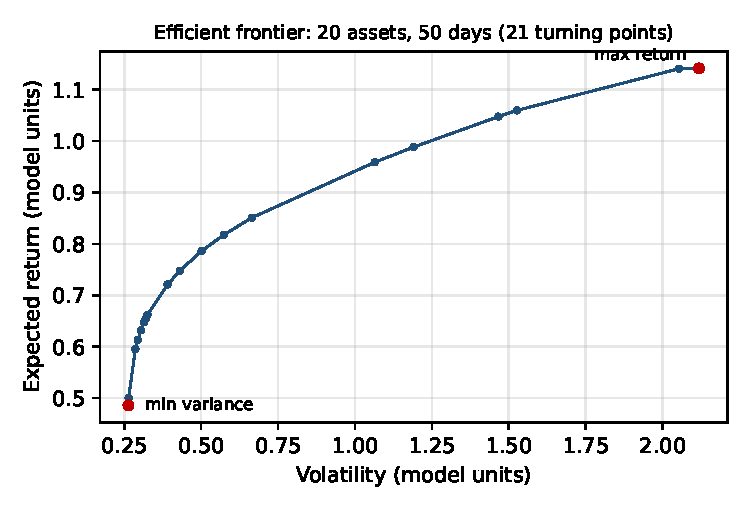
\includegraphics[width=0.72\textwidth]{frontier.pdf}
\caption{The efficient frontier of the $20$-asset, $50$-day problem in
expected-return / volatility space, computed exactly by the Critical Line
Algorithm. Each marker is one of the $21$ turning points; the endpoints are the
maximum-return portfolio ($\lambda=\infty$) and the global minimum-variance
portfolio ($\lambda=0$). Axes are in the dimensionless ``model units'' of the
simulated factor model (per-period return and volatility of the synthetic
process); unlike the annualised S\&P 500 frontier of
Figure~\ref{fig:realfrontier}, they carry no calendar scale and are meaningful
only relative to one another.}
\label{fig:frontier}
\end{figure}

\subsection{Runtime versus problem size}
\label{sec:scaling}

We next trace the full frontier for $n \in \{20, 40, 80, 160, 320, 640\}$ assets,
each from a ground-truth $K = 10$ factor model so that the dense and factor
backends again solve the identical $\Sig$ and return the same frontier. For
reference we also time the \texttt{CLA} of PyPortfolioOpt \citep{pyportfolioopt},
a widely-used implementation of the critical-line algorithm of
\citet{bailey2013}, on the same dense problem. The number of turning points tracks $n$ closely
($21, 42, 81, 159, 322, 641$ respectively, and PyPortfolioOpt finds essentially
the same set), confirming the $O(n)$ count of \S\ref{sec:experiment}. The two
implementations also agree numerically: their minimum-variance portfolios (the
$\lambda = 0$ endpoint, which is unique for a positive-definite $\Sig$) match to
machine precision, differing by at most $\sim\!10^{-16}$ in any weight across these
problems.

Figure~\ref{fig:scaling} plots the median trace time against $n$ on log--log
axes. A least-squares fit over the largest four sizes gives an empirical exponent
of $\approx 2.2$ for the \texttt{cvxcla} dense backend and $\approx 1.3$ for the
factor backend: the dense per-iteration solve scales like $O(n_\F^3)$ over $O(n)$
iterations, while the Woodbury solve with fixed $K$ stays close to linear in $n$.
The dense and factor backends are comparable for small universes (the Woodbury
correction carries a fixed $K\times K$ overhead), but the factor backend pulls
away as $n$ grows: from rough parity at $n=40$ to a $\approx 9\times$ speedup
at $n=640$ (Table~\ref{tab:scaling}). This $\approx 9\times$ is the genuine
\emph{algorithmic} gain: both backends are vectorised \texttt{numpy} solving the
identical $\Sig$, so the only difference is the asymptotic Woodbury advantage of
the structured solve over the dense one.

For external context we also time PyPortfolioOpt, which scales far more steeply
($\approx n^{3.4}$): at $n=640$ it takes about $261$~seconds, so \texttt{cvxcla}'s
dense backend is roughly $324\times$ faster and the factor backend roughly
$2980\times$ faster. This gap is not a \texttt{numpy}-versus-Python artefact (
PyPortfolioOpt uses \texttt{numpy} for its linear algebra) but a consequence of
how it organises the work: it rebuilds a full free-block inverse at every step,
and once per candidate in the asset-entry search (\S\ref{sec:bailey}).
\S\ref{sec:baseline} separates this structural cost from the genuinely
\emph{algorithmic} advantage, which is the structured factor backend.

\begin{table}[h]
\centering
\begin{tabular}{rrrrrr}
\toprule
$n$ & Turning points & PyPortfolioOpt [ms] & Inverse baseline [ms] & \texttt{cvxcla} dense [ms] & \texttt{cvxcla} factor [ms] \\
\midrule
$20$  & $21$  & $10.6$       & $0.7$   & $1.3$   & $1.4$ \\
$40$  & $42$  & $41.0$       & $1.9$   & $3.3$   & $3.1$ \\
$80$  & $81$  & $216.6$      & $4.8$   & $7.8$   & $6.5$ \\
$160$ & $159$ & $1{,}550$    & $13.6$  & $23.4$  & $13.9$ \\
$320$ & $322$ & $16{,}789$   & $49.9$  & $111.3$ & $33.5$ \\
$640$ & $641$ & $261{,}335$  & $337.9$ & $805.8$ & $87.7$ \\
\bottomrule
\end{tabular}
\caption{Frontier trace time versus number of assets $n$ ($K=10$ factors). All
four implementations are timed with the \emph{same} protocol (the median of
$3$ repetitions on the same machine and inputs) and return the same
$O(n)$-point frontier. ``Inverse baseline'' is the incremental-inverse CLA of
\S\ref{sec:baseline} (\srcfile{experiments/inverse_cla.py}{experiments/inverse\_cla.py}): it shares
\texttt{cvxcla}'s vectorised event logic but maintains $\Sig_{\F\F}\inv$ through
rank-one updates instead of re-solving each step, so the gap between it and the
dense backend isolates the linear-algebra strategy. Empirically the times scale
like $\approx n^{3.4}$ (PyPortfolioOpt), $\approx n^{2.0}$ (inverse baseline),
$\approx n^{2.2}$ (\texttt{cvxcla} dense) and $\approx n^{1.3}$
(\texttt{cvxcla} factor).}
\label{tab:scaling}
\end{table}

\begin{figure}[h]
\centering
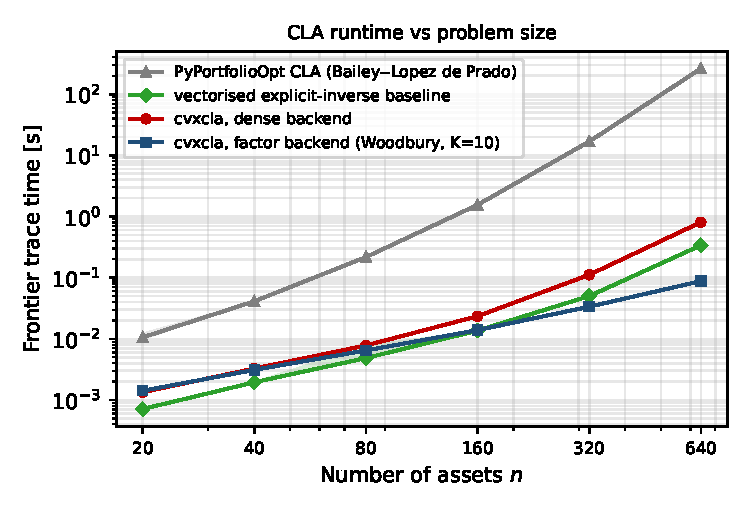
\includegraphics[width=0.72\textwidth]{scaling.pdf}
\caption{Frontier trace time as a function of the number of assets $n$ (log--log).
PyPortfolioOpt \citep{pyportfolioopt}, a critical-line implementation in pure
Python, scales like $\approx n^{3.4}$; the vectorised explicit-inverse baseline of
\S\ref{sec:baseline} like $\approx n^{2.0}$; \texttt{cvxcla}'s dense backend like
$\approx n^{2.2}$; and its diagonal-plus-low-rank factor backend, solving the
identical covariance through the Woodbury identity, like $\approx n^{1.3}$. At
$n = 640$ the factor backend is roughly $2980\times$ faster than PyPortfolioOpt and
$9\times$ faster than the dense backend. The incremental-inverse baseline and the
dense backend lie close together, far below PyPortfolioOpt. Markers are the
median of $3$ repetitions; the shaded band around each spans their min and max.}
\label{fig:scaling}
\end{figure}

\subsection{What the runtime gap is, and is not}
\label{sec:baseline}

The $\approx 324\times$ gap between \texttt{cvxcla}'s dense backend and
PyPortfolioOpt at $n=640$ invites a lazy explanation (``vectorised
\texttt{numpy} versus slow Python'') that is wrong. PyPortfolioOpt already uses
\texttt{numpy} (\texttt{np.linalg.inv}, \texttt{np.dot}) for its per-step linear
algebra. It is slow because of \emph{how} it organises the work: it rebuilds a full
inverse of the free block from scratch at every step, and in the branch that
decides which blocked asset should re-enter it recomputes that full $O(n_\F^3)$
inverse once for \emph{every} candidate blocked asset, of order $n$ dense
inverses per turning point. \texttt{cvxcla} instead forms the affine segment once
per step from a single solve and evaluates all event candidates simultaneously
(the $L$ matrix of \S\ref{sec:events}), so the gap is structural and algorithmic,
not a \texttt{numpy} artefact.

That still leaves a fair question about \texttt{cvxcla}'s own dense backend: it too
re-solves from scratch each step, discarding the previous factorisation. Could a
CLA that instead \emph{maintains} the free-block inverse and updates it by
rank-one formulas do better? We test exactly this with a third implementation
(\srcfile{experiments/inverse_cla.py}{experiments/inverse\_cla.py}): a CLA that shares \texttt{cvxcla}'s
vectorised event logic but maintains $\Sig_{\F\F}\inv$ through rank-one bordered
(asset enters) and deletion (asset leaves) updates, $O(n_\F^2)$ per step against
the fresh solve's $O(n_\F^3)$. It is \emph{not} a reimplementation of
PyPortfolioOpt (it avoids PyPortfolioOpt's per-candidate rebuild) and it
traces the identical turning points to machine precision (max.\ weight discrepancy
$<10^{-13}$ across $n=20$--$160$), so the comparison against the dense backend is
clean: only the linear-algebra strategy differs.

The answer is yes: the incremental-inverse baseline ($\approx n^{2.0}$, $338$~ms at
$n=640$) is about $2.4\times$ \emph{faster} than the dense backend
($\approx n^{2.2}$, $806$~ms), exactly as the $O(n_\F^2)$-versus-$O(n_\F^3)$ count
predicts. \texttt{cvxcla}'s block elimination is therefore not the fastest possible
dense strategy, and the package ships the incremental inverse as the opt-in
\texttt{IncrementalDenseCovariance} backend (\S\ref{sec:incremental}) for callers
who want that win. It is not the \emph{default} because the fresh solve is what
composes cleanly with the covariance operator (\S\ref{sec:operators}) and is
numerically robust step to step: the factor backend never forms $\Sig_{\F\F}$ at
all, so there is no inverse to maintain: it solves through the Woodbury
identity. The default dense backend gives up the modest incremental-inverse win to
keep one turning-point loop that runs over \emph{any} backend, and the factor
backend more than repays it: at $n=640$ it is $\approx 9.2\times$ faster than the
dense backend and $\approx 3.9\times$ faster than the incremental-inverse baseline,
the only one of the four implementations with a genuinely sub-quadratic exponent
($\approx n^{1.3}$). The structured solve, not the linear-algebra bookkeeping, is
the real algorithmic advance.

\subsection{Runtime versus factor rank}
\label{sec:rankscaling}

The advantage of the factor backend is not unconditional: it comes from the
low-rank structure, so it must fade as the rank $K$ approaches $n$. To make this
precise we fix the universe at $n = 320$ assets and vary the number of factors
$K \in \{20, 40, 80, 160, 320\}$ of the ground-truth covariance, tracing the same
frontier with both backends. The dense backend factorises the same $320 \times
320$ free block regardless of $K$, so its time is essentially flat; the Woodbury
solve costs $O(n_\F K^2 + K^3)$ per step and grows with $K$. Figure~\ref{fig:rank}
and Table~\ref{tab:rank} show the crossover: the factor backend is $3.1\times$
faster at $K=20$, reaches parity near $K=160$, and is about $2\times$ \emph{slower}
at $K = 320$, where the ``low-rank'' part is full rank and the Woodbury correction
is pure overhead. The practical reading is that the structured backend pays off
precisely in the regime real risk models inhabit: a few tens of factors over
hundreds or thousands of assets ($K \ll n$).

\begin{table}[h]
\centering
\begin{tabular}{rrrr}
\toprule
$K$ & \texttt{cvxcla} dense [ms] & \texttt{cvxcla} factor [ms] & Speedup \\
\midrule
$20$  & $112.0$ & $36.2$  & $3.1\times$ \\
$40$  & $114.1$ & $43.0$  & $2.7\times$ \\
$80$  & $108.1$ & $59.7$  & $1.8\times$ \\
$160$ & $86.4$  & $78.5$  & $1.1\times$ \\
$320$ & $87.1$  & $194.4$ & $0.4\times$ \\
\bottomrule
\end{tabular}
\caption{Frontier trace time at fixed $n = 320$ as the factor rank $K$ varies
(median of $3$ repetitions). The dense backend is independent of $K$; the
Woodbury backend grows with $K$ and loses its advantage once $K$ is no longer
small relative to $n$. Both return the same $\approx 320$-point frontier.}
\label{tab:rank}
\end{table}

\begin{figure}[h]
\centering
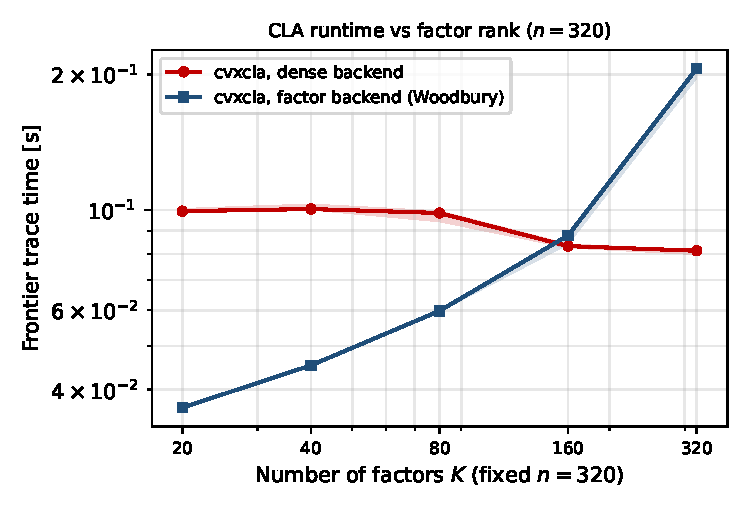
\includegraphics[width=0.72\textwidth]{rank_scaling.pdf}
\caption{Frontier trace time at fixed $n = 320$ as a function of the factor rank
$K$ (log--log). The dense backend is flat in $K$; the diagonal-plus-low-rank
factor backend grows like the Woodbury cost $O(n_\F K^2 + K^3)$ and crosses the
dense line near $K \approx 160$. The structured backend wins only while
$K \ll n$. Markers are the median of $3$ repetitions; the shaded band spans
their min and max.}
\label{fig:rank}
\end{figure}

\subsection{Exactness against a reference QP solver}
\label{sec:exactness}

The frontier is claimed to be \emph{exact}: each segment \eqref{eq:segment} is the
true optimiser of \eqref{eq:qp}, not an interpolation. We verify this
independently. Taking $40$ real assets (\S\ref{sec:empirical}, full-history
sample covariance, condition number $\approx 200$), we trace the frontier with
the CLA ($29$ turning points) and then, at the midpoint $\lambda$ of every one of
the $27$ interior segments, re-solve the parametric quadratic program
\eqref{eq:qp} from scratch with a general convex solver (CVXPY/Clarabel
\citep{cvxpy}, tight tolerances) and compare its optimiser against the CLA weights
read off the segment by linear interpolation in $\lambda$. The agreement is at
solver precision (median weight discrepancy $5\times 10^{-8}$, maximum
$1.3\times 10^{-5}$) confirming that the affine segments coincide with the QP
optima rather than approximating them (\srcfile{experiments/validate_exact.py}{experiments/validate\_exact.py}).

\subsection{Empirical example: the S\&P 500 frontier}
\label{sec:empirical}

To close, we run the algorithm on real data. The experiment runs off a frozen
snapshot shipped with the package,
\srcfile{experiments/data/sp500_pct_returns.parquet}{experiments/data/sp500\_pct\_returns.parquet}
($N = 494$ assets over $T = 1213$ trading days, 2021-07-30 to 2026-05-29;
SHA-256 \texttt{b5faa522\ldots9937e}), so the figures below reproduce
deterministically and offline, with no dependence on a live data feed. The
snapshot was produced once by
\srcfile{experiments/fetch_sp500.py}{experiments/fetch\_sp500.py}, which pulls the
then-current S\&P 500 constituents from Wikipedia, downloads five years of daily
adjusted-close prices via \texttt{yfinance}, and drops thinly-traded names; that
script is retained for provenance and refresh only and is not part of the
reproducible path. From the
full-history sample mean and covariance (condition number $\approx 1.1\times
10^{5}$) the CLA traces the entire long-only frontier (\textbf{96 turning
points}) in a median of $\approx 14$~ms (Figure~\ref{fig:realfrontier}); a
rank-$20$ diagonal-plus-low-rank approximation of the same covariance traces a
near-identical frontier ($89$ turning points) in $\approx 9$~ms through the
Woodbury backend. The annualised frontier spans expected returns of
$0.14$--$0.89$ over volatilities of $0.10$--$0.87$, with a maximum Sharpe ratio of
about $2.7$. This figure is measured in-sample (the frontier is optimised over
the same sample mean and covariance from which it is computed) and so overstates
what is achievable out-of-sample; it is reported only to characterise the geometry
of the frontier on a realistic problem, not as a claim of attainable performance.

\begin{figure}[h]
\centering
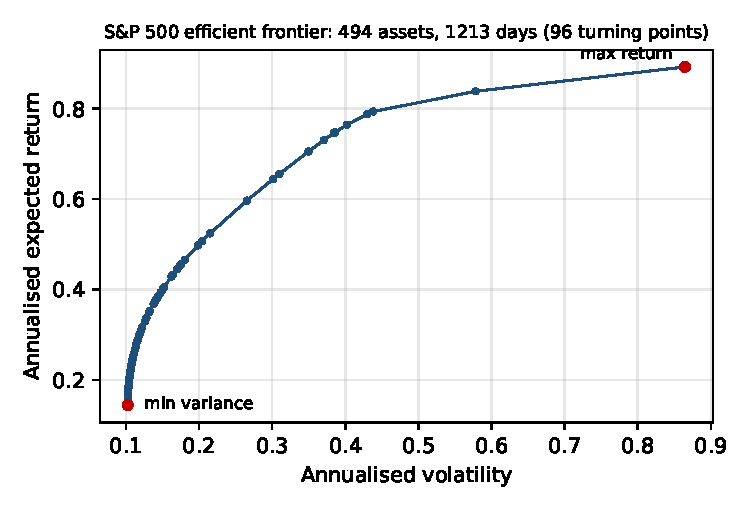
\includegraphics[width=0.72\textwidth]{real_frontier.pdf}
\caption{The long-only efficient frontier of $494$ S\&P 500 constituents from a
full-history daily sample covariance ($T = 1213$ days), computed exactly by the
CLA. Moments are annualised; each marker is one of the $96$ turning points.}
\label{fig:realfrontier}
\end{figure}

\paragraph{A real degeneracy, diagnosed and repaired.}
The traces above run cleanly because the expected returns are well separated and
the covariance is well conditioned. Near-degenerate inputs are more delicate, and
earlier versions of the algorithm aborted on them. The cause is now understood,
and it is neither a conditioning nor a rank failure in the usual sense. On a
near-rank-deficient covariance the smallest eigenvalues span near-flat directions
of the objective; accumulated floating-point round-off over the hundreds of
turning points of a large trace nudges a free weight a hair (typically $10^{-5}$
to $10^{-3}$) outside its box along one of those directions. The candidate is
therefore optimal to solver precision but not exactly feasible, and a strict
feasibility check rejects it.

Because the deviation lies in the covariance's flat directions, projecting the
candidate back onto the feasible box (and rescaling to restore the budget)
changes the objective only at the level of the round-off itself. The
implementation does exactly this in \texttt{\_emit}, and the trace then completes
with turning points that remain optimal: across a controlled rank-deficiency
sweep every completed point matches a reference QP solve (CVXPY/Clarabel,
\S\ref{sec:exactness}) in objective to $\sim\!10^{-8}$
(Figure~\ref{fig:degeneracy}), and the full-history frontier of
\S\ref{sec:empirical} is unchanged to the last digit, since well-posed turning
points are already strictly feasible and the projection is then a no-op. The
short-window S\&P 500 covariances that previously aborted now trace to
completion.

The repair is deliberately bounded, and the two regimes are told apart by the
\emph{conditioning} of the free-asset block, not by the size of the violation it
happens to produce. While that block stays numerically full rank its solve is
reliable and any infeasibility is round-off, which is projected away; once the
free set grows past the covariance rank the block is numerically singular and its
solve is unreliable, so projecting whatever it returns could silently yield a
suboptimal frontier. A guard therefore declines as soon as the free block's
reciprocal condition number falls below $10^{-12}$ (the conventional
numerical-singularity scale), raising an actionable diagnosis instead. We key the
guard on conditioning rather than on the box violation because the violation is
the residual of a singular solve and its magnitude varies with the BLAS/LAPACK
build, whereas the conditioning is read from the block's symmetric eigenvalues
and is identical on every platform. This is the precise guarantee \emph{for rank
and conditioning degeneracy}: while the free-asset block stays full rank the trace
completes and every turning point is optimal; when it does not, the algorithm
declines rather than mislead. It speaks to the linear algebra, not to event ties:
the distinct, combinatorial degeneracy of many events coincident at one
$\lambda^{\star}$ is handled by the Bland-style tie-break of \S\ref{sec:bland},
which is robust on the degenerate problems we test but, like the worst-case
turning-point count, is not proven to cover every adversarial tie-heavy or very
large instance. A
well-conditioned, full-rank estimate (ample history, or a structured
\texttt{FactorCovariance}, which is positive definite by construction) stays in
the first regime. The experiment is reproducible from
\srcfile{experiments/degeneracy_boundary.py}{experiments/degeneracy\_boundary.py}.

\begin{figure}[h]
\centering
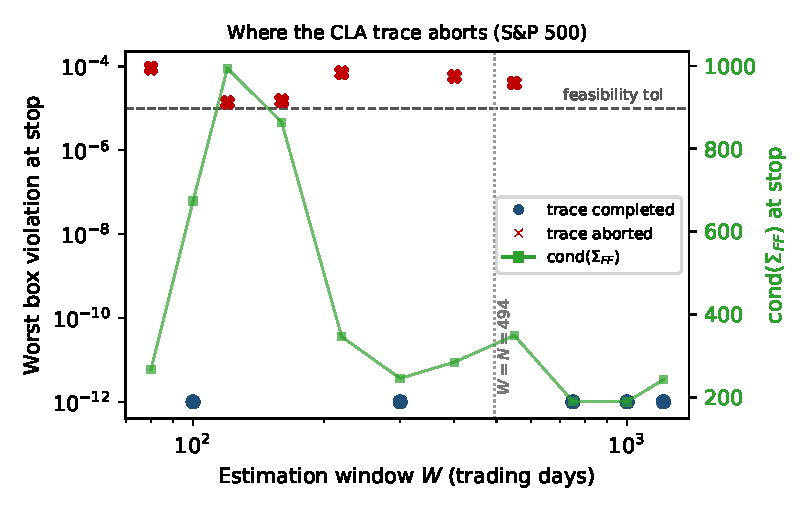
\includegraphics[width=0.72\textwidth]{degeneracy.pdf}
\caption{A controlled rank-deficiency sweep at $n = 120$: the sample covariance
is estimated from $T$ observations, so its rank is $\approx \min(T-1, n)$ and
falls as $T$ shrinks (leftward). Each marker is the worst conditioning (2-norm
condition number) of a \emph{candidate} turning point's free-asset block. Blue
circles complete the full trace, and every completed frontier is optimal,
matching a reference QP in objective to $\sim\!10^{-8}$. Red crosses are declined.
Completions sit far below the singularity guard (dashed, condition number
$10^{12}$): their free blocks stay numerically full rank (condition number
$\lesssim 10^{3}$), so the only infeasibility is round-off in the covariance's
near-flat directions, repaired by projecting onto the feasible box. Declines sit
far above it (condition number $\sim\!10^{16}$): the free set has grown past the
covariance rank, the block is numerically singular and its solve is unreliable,
so the algorithm declines rather than risk a suboptimal frontier. The boundary is
monotone in $T$, and the wide gap between the two regimes leaves the guard
threshold uncritical.}
\label{fig:degeneracy}
\end{figure}

\section{Connection to homotopy methods: least angle regression and the LASSO}
\label{sec:lars}

The CLA is one instance of a broader idea that recurs across optimisation and
statistics: when the optimiser of a convex problem is followed as a single scalar
parameter varies, the solution path is frequently piecewise linear, and it can be
traced exactly by stepping from one breakpoint to the next while maintaining an
active set. The same structure drives least angle regression (LARS) and the LASSO
homotopy in statistical learning \citep{tibshirani1996, osborne2000, efron2004}.
Making the correspondence explicit places the CLA in a family it is seldom
presented alongside, and separates the features that are essential to the method
from those particular to the portfolio setting.

The most direct relative is in control rather than statistics. The CLA is a
one-parameter \emph{multi-parametric quadratic program} (mpQP): a strictly convex
QP whose linear term depends affinely on a parameter, and whose solution map is
therefore piecewise affine over a polyhedral partition of the parameter space. This
is the structure exploited by explicit model predictive control, where the optimal
control law is precomputed as a piecewise-affine function of the state by mpQP
path-following \citep{bemporad2002, tondel2003}. The turning points of the CLA are
the breakpoints of that map for the single risk-aversion parameter, and the event
logic of \S\ref{sec:events} is the one-dimensional specialisation of the
critical-region traversal used there. The general mpQP machinery also handles
arbitrary polyhedral constraints, and \texttt{cvxcla} admits them too, through the
inequality rows $G w \le h$ of \eqref{eq:qp}. The mechanism is the row analogue of
the box active set. A box bound is a per-variable inequality: an asset is free or
blocked, and the events are a free weight reaching a bound or a blocked multiplier
releasing it. A row of $G w \le h$ is a per-row inequality: it is active (held at
$g_i\trans w = h_i$) or slack, and the events are a slack row's residual reaching
zero, so it activates, or an active row's multiplier reaching zero, so it releases.
Both kinds of event are the same ``smallest positive ratio to the next breakpoint''
along the affine segment; the row events are simply scanned over the $p$ rows of $G$
in addition to the $n$ box coordinates (\S\ref{sec:events}).

Crucially, this does \emph{not} sacrifice the structure that the equality-only case
enjoys. An active inequality row enters the reduced KKT system \eqref{eq:kkt} exactly
as an equality row does: stacking $C = [\,A;\,G_{\Sset}\,]$ over the active rows
recovers the equality-only solve with $A$ replaced by $C$, so each step is still a
solve against the free covariance block $\Sig_{\F\F}$ (through the operator interface
of \S\ref{sec:operators}, never an $n\times n$ matrix) feeding an
$(m+|\Sset|)\times(m+|\Sset|)$ Schur complement. The box bounds remain a separate,
cheaper per-variable active set rather than being folded into $G$, so the common
box-only problem pays nothing for the generalisation.

What does \emph{not} work, and is worth recording because it is the natural first
reflex, is turning an inequality into an equality with a slack. Writing
$g_i\trans w + s_i = h_i$ with $s_i \ge 0$ leaves the slack with no curvature in the
objective, so the augmented Hessian $\operatorname{diag}(\Sig, 0)$ is only positive
\emph{semi}-definite and the reduced solve is singular whenever a slack is free
(precisely when its inequality is inactive). Admitting general inequalities therefore
goes through the bordered system above and a per-row event, not a change of
variables, which is exactly what the implementation does.

The LASSO solves, for a response $y$ and design matrix $X$,
\[
\min_{\beta}\ \tfrac12\,\|y - X\beta\|_2^2 \;+\; \lambda\,\|\beta\|_1,
\]
and its minimiser $\beta(\lambda)$ is a continuous, piecewise-linear function of the
penalty $\lambda$ \citep{efron2004, rosset2007}. As $\lambda$ decreases from the
value at which $\beta = 0$ towards $0$, the path proceeds in straight segments; at
each breakpoint the active set (the support of $\beta$) changes, either because an
inactive variable whose correlation with the current residual reaches $\lambda$
enters, or because an active coefficient reaches zero and leaves. LARS computes
these breakpoints and segment directions directly, exactly as the CLA computes
turning points and the affine segments \eqref{eq:segment} between them.

The two algorithms line up term for term (Table~\ref{tab:lars}).

\begin{table}[h]
\centering
\begin{tabular}{lll}
\toprule
Ingredient & Critical Line Algorithm & LARS / LASSO homotopy \\
\midrule
Swept parameter & risk aversion $\lambda:\infty\!\to\!0$ & penalty $\lambda:\infty\!\to\!0$ \\
Solution path   & $w(\lambda)=\alpha+\lambda\beta$ (pw.\ linear) & $\beta(\lambda)$ (pw.\ linear) \\
Active set      & free set $\F$ (weights off the bounds) & support (nonzero $\beta_j$) \\
Linear solve    & reduced KKT over $\Sig_{\F\F}$ & least squares over $X_{\mathcal A}$ \\
Enter event     & blocked multiplier changes sign & residual correlation reaches $\lambda$ \\
Leave event     & free weight reaches a box bound & active coefficient reaches zero \\
Step length     & smallest positive ratio to next event & smallest positive step to next breakpoint \\
Degeneracy      & Bland lowest-index tie-break (\S\ref{sec:bland}) & tie-break among simultaneous hits \\
\bottomrule
\end{tabular}
\caption{The Critical Line Algorithm and the LARS/LASSO homotopy as two instances
of the same parametric active-set scheme. The role played by the covariance $\Sig$
and the mean $\mu$ in the reduced KKT solve \eqref{eq:saddle} is played by the Gram
matrix $X\trans X$ and the vector $X\trans y$ in the regression path.}
\label{tab:lars}
\end{table}

The correspondence is not a coincidence. \citet{rosset2007} characterise when a
regularised solution path is piecewise linear: a quadratic (or piecewise-quadratic)
loss together with a polyhedral, i.e.\ piecewise-linear, constraint or penalty
suffices. Both problems meet the criterion. The CLA minimises a quadratic objective
\eqref{eq:qp} over a polyhedral feasible set (box bounds, linear equalities, and
linear inequalities); the
LASSO minimises a quadratic loss under a polyhedral ($\ell_1$) penalty. In each case
the KKT conditions are affine in the parameter, the system matrix is constant while
the active set is fixed, and the active set can change only at the discrete
parameter values that the homotopy steps between. The ``smallest positive ratio to
the next event'' rule of \S\ref{sec:events} is the same step-length computation that
advances the LARS path, and both inherit it, for the same anti-cycling reasons, from
the simplex method (\S\ref{sec:bland}).

Three differences are worth stating precisely, since they are exactly what
distinguishes the portfolio problem.

\paragraph{What induces the active set.} In the CLA the active set is carved out by
\emph{explicit} polyhedral constraints: an asset is blocked when it sits on a box
bound, and the events are free weights reaching those bounds, or blocked multipliers
releasing them. In the LASSO the active set is \emph{induced} by the $\ell_1$
penalty through its subgradient: sparsity is an emergent property of the geometry,
not a constraint the modeller writes down. The same polyhedral mechanism runs in
opposite directions, one imposing the faces and the other discovering them.

\paragraph{Entering and leaving.} Forward LARS only ever \emph{adds} variables to
the active set; the LASSO modification restores the ability to drop one when its
coefficient crosses zero. The CLA needs both moves throughout, as assets become free
and blocked while $\lambda$ decreases, so it corresponds to the full LASSO homotopy
rather than to forward LARS.

\paragraph{The data enter only through linear algebra.} The Gram matrix $X\trans X$
that defines the LARS direction is played here by the covariance $\Sig$ in the
reduced KKT solve \eqref{eq:saddle}, and $X\trans y$ by the expected-return vector
$\mu$. Seen this way, the covariance-operator abstraction of \S\ref{sec:operators} is
the statement that the path-tracing logic touches $\Sig$ only through a few
linear-algebraic operations, just as the LARS recursion touches $X$ only through
Gram-matrix solves; a structured $\Sig$ (a factor model) is the portfolio analogue
of a structured or kernelised design. The package makes the correspondence literal:
the \texttt{GramCovariance} backend (\S\ref{sec:gram}) builds $\Sig$ from the
centred data matrix $X_c$ directly through \eqref{eq:gram}, so the CLA runs off
$X_c$ exactly as LARS runs off the design matrix, and the protocol it calls is named
\texttt{QuadraticForm} rather than after the covariance for this reason.

The bridge is more than analogy. \citet{brodie2009} add a gross-exposure constraint
$\|w\|_1 \le c$ to the Markowitz problem and show that the result \emph{is} a LASSO,
with $c$ promoting sparse, stable portfolios. For the long-only, fully-invested
problem this constraint is silent, since the budget already fixes $\|w\|_1 =
\mathbf{1}\trans w = 1$, which is why the plain CLA traces a frontier rather than a
sparsity path. Once short positions are admitted under a gross-exposure cap,
however, the parametric program the CLA traces and the LASSO path coincide: the two
are then not merely structurally similar but two homotopies over the same parametric
quadratic program.

\section{Conclusion}

The Critical Line Algorithm computes the complete mean--variance efficient frontier by
recognising its piecewise-linear structure in weight space and walking from the
maximum-return portfolio to the minimum-variance portfolio, flipping one asset between
the free and blocked sets at each turning point. The \texttt{cvxcla} implementation
realises each step as a single block-eliminated KKT solve, hardens the event logic
against degeneracy and floating-point noise, and abstracts the covariance behind a
small operator protocol so that structured risk models obtain the same exact frontier
without ever forming the dense matrix, and at a fraction of its cost when their
structure is genuinely low-rank. The same parametric active-set mechanism places the
CLA alongside multi-parametric quadratic programming and the LARS/LASSO homotopy: the
operator interface is what lets one path-tracing engine serve both the portfolio
frontier and, with the covariance replaced by a Gram matrix, a LASSO regularisation
path.

The Critical Line Algorithm is Markowitz's, and this paper claims none of it as new.
Seven decades on, it remains the only method that computes the entire mean--variance
frontier exactly rather than sampling it, and our aim has been to give it a modern,
open, and structured home rather than to improve upon it. The work is, in that sense, a
bow to Harry Markowitz (1927--2023), who gave the field both the question and its
constructive answer.

\section*{Acknowledgements}
\addcontentsline{toc}{section}{Acknowledgements}

The author thanks Stephen Boyd and Philipp Schiele. The first versions of the
solver were implemented while the author stayed for a sabbatical at Boyd's group
at Stanford University.

\begin{thebibliography}{9}

\bibitem[Markowitz(1952)]{markowitz1952}
H.~M. Markowitz.
\newblock Portfolio selection.
\newblock \emph{The Journal of Finance}, 7(1):77--91, 1952.

\bibitem[Markowitz(1956)]{markowitz1956}
H.~M. Markowitz.
\newblock The optimization of a quadratic function subject to linear constraints.
\newblock \emph{Naval Research Logistics Quarterly}, 3(1--2):111--133, 1956.

\bibitem[Markowitz(1959)]{markowitz1959}
H.~M. Markowitz.
\newblock \emph{Portfolio Selection: Efficient Diversification of Investments}.
\newblock John Wiley \& Sons, New York, 1959.

\bibitem[Markowitz et~al.(2021)]{markowitz2021}
H.~Markowitz, D.~Starer, H.~Fram, and S.~Gerber.
\newblock Avoiding the downside: A practical review of the critical line
algorithm for mean--semivariance portfolio optimization.
\newblock In \emph{Handbook of Applied Investment Research}, chapter~17. World
Scientific, 2021.
\newblock \url{https://doi.org/10.1142/9789811222634_0017}.

\bibitem[Niedermayer and Niedermayer(2010)]{niedermayer2010}
A.~Niedermayer and D.~Niedermayer.
\newblock Applying Markowitz's critical line algorithm.
\newblock In \emph{Handbook of Portfolio Construction}, pages 383--400. Springer, 2010.

\bibitem[Bailey and L\'opez de Prado(2013)]{bailey2013}
D.~H. Bailey and M.~L\'opez de Prado.
\newblock An open-source implementation of the critical-line algorithm for portfolio
optimization.
\newblock \emph{Algorithms}, 6(1):169--196, 2013.

\bibitem[Martin(2021)]{pyportfolioopt}
R.~A. Martin.
\newblock {PyPortfolioOpt}: portfolio optimization in {Python}.
\newblock \emph{Journal of Open Source Software}, 6(61):3066, 2021.
\newblock \url{https://doi.org/10.21105/joss.03066}.

\bibitem[Diamond and Boyd(2016)]{cvxpy}
S.~Diamond and S.~Boyd.
\newblock {CVXPY}: a {Python}-embedded modeling language for convex optimization.
\newblock \emph{Journal of Machine Learning Research}, 17(83):1--5, 2016.

\bibitem[Wolfe(1959)]{wolfe1959}
P.~Wolfe.
\newblock The simplex method for quadratic programming.
\newblock \emph{Econometrica}, 27(3):382--398, 1959.

\bibitem[Sharpe(1963)]{sharpe1963}
W.~F. Sharpe.
\newblock A simplified model for portfolio analysis.
\newblock \emph{Management Science}, 9(2):277--293, 1963.

\bibitem[Perold(1984)]{perold1984}
A.~F. Perold.
\newblock Large-scale portfolio optimization.
\newblock \emph{Management Science}, 30(10):1143--1160, 1984.

\bibitem[Markowitz and Todd(2000)]{markowitz2000}
H.~M. Markowitz and G.~P. Todd.
\newblock \emph{Mean-Variance Analysis in Portfolio Choice and Capital Markets}.
\newblock Frank J. Fabozzi Associates, New Hope, PA, 2000.

\bibitem[Stein et~al.(2008)]{stein2008}
M.~Stein, J.~Branke, and H.~Schmeck.
\newblock Efficient implementation of an active set algorithm for large-scale
portfolio selection.
\newblock \emph{Computers \& Operations Research}, 35(12):3945--3961, 2008.

\bibitem[Hirschberger et~al.(2010)]{hirschberger2010}
M.~Hirschberger, Y.~Qi, and R.~E. Steuer.
\newblock Large-scale MV efficient frontier computation via a procedure of
parametric quadratic programming.
\newblock \emph{European Journal of Operational Research}, 204(3):581--588, 2010.

\bibitem[Tibshirani(1996)]{tibshirani1996}
R.~Tibshirani.
\newblock Regression shrinkage and selection via the lasso.
\newblock \emph{Journal of the Royal Statistical Society, Series B}, 58(1):267--288, 1996.

\bibitem[Osborne et~al.(2000)]{osborne2000}
M.~R. Osborne, B.~Presnell, and B.~A. Turlach.
\newblock A new approach to variable selection in least squares problems.
\newblock \emph{IMA Journal of Numerical Analysis}, 20(3):389--403, 2000.

\bibitem[Efron et~al.(2004)]{efron2004}
B.~Efron, T.~Hastie, I.~Johnstone, and R.~Tibshirani.
\newblock Least angle regression.
\newblock \emph{The Annals of Statistics}, 32(2):407--499, 2004.

\bibitem[Rosset and Zhu(2007)]{rosset2007}
S.~Rosset and J.~Zhu.
\newblock Piecewise linear regularized solution paths.
\newblock \emph{The Annals of Statistics}, 35(3):1012--1030, 2007.

\bibitem[Brodie et~al.(2009)]{brodie2009}
J.~Brodie, I.~Daubechies, C.~De~Mol, D.~Giannone, and I.~Loris.
\newblock Sparse and stable Markowitz portfolios.
\newblock \emph{Proceedings of the National Academy of Sciences}, 106(30):12267--12272, 2009.

\bibitem[Bemporad et~al.(2002)]{bemporad2002}
A.~Bemporad, M.~Morari, V.~Dua, and E.~N. Pistikopoulos.
\newblock The explicit linear quadratic regulator for constrained systems.
\newblock \emph{Automatica}, 38(1):3--20, 2002.

\bibitem[T\o ndel et~al.(2003)]{tondel2003}
P.~T\o ndel, T.~A. Johansen, and A.~Bemporad.
\newblock An algorithm for multi-parametric quadratic programming and explicit MPC solutions.
\newblock \emph{Automatica}, 39(3):489--497, 2003.

\end{thebibliography}

\end{document}
